% mpsub.tex -- Computational Optimization and Applications (COAP) format
% Document class: svjour3 (Springer format for COAP)
\RequirePackage{fix-cm}
\documentclass[smallextended]{svjour3}

\smartqed  % flush right qed marks, e.g. at end of proof

\journalname{Computational Optimization and Applications}

% Packages
\usepackage[T1]{fontenc}
\usepackage{amsmath}
\usepackage{amssymb}
\usepackage{amsfonts}
\usepackage{graphicx}
\usepackage{booktabs}
\usepackage{multirow}
\usepackage{algorithm}
\usepackage{algorithmic}
\usepackage{bm}
\usepackage{mathtools}
\usepackage{url}
\usepackage{marvosym}
\usepackage{hyperref}
\newcommand{\doi}[1]{\url{https://doi.org/#1}}

% Theorem-like environments
\spdefaulttheorem{assumption}{Assumption}{\bfseries}{\itshape}

% Running headers
\titlerunning{MpSub: subspace trust-region derivative-free LLM fine-tuning}
\authorrunning{Y.~Wang, H.~Yao, and P.~Xie}

%%%%%%%%%%% Custom macros %%%%%%%%%%%
\newcommand{\bx}{\bm{x}}
\newcommand{\dd}{\bm{d}}
\newcommand{\B}{\bm{B}}
\newcommand{\bP}{\bm{P}}
\newcommand{\bd}{\bm{d}}
\newcommand{\bg}{\bm{g}}
\newcommand{\bz}{\bm{z}}
\newcommand{\bs}{\bm{s}}
\providecommand{\coloneqq}{\mathrel{\mathop:}=}
%%%%%%%%%%%

\begin{document}

\title{MpSub: A Momentum $p$-Dimensional Subspace Trust-Region Method for Derivative-Free Fine-Tuning of Large Language Models}

\author{Yuyang Wang \and Haoyu Yao \and \mbox{Pengcheng Xie}}

\institute{Y. Wang \and H. Yao \at
              Xi'an Jiaotong University, Xi'an, China \\
              \email{vibrancy05@stu.xjtu.edu.cn, yaohaoyu@stu.xjtu.edu.cn}
           \and
           P. Xie (\Letter) \at
              Lawrence Berkeley National Laboratory, Berkeley, CA, USA \\
              \email{pxie@lbl.gov}
}

\date{Received: date / Accepted: date}

\maketitle

\begin{abstract}
Zeroth-order optimization avoids the activation memory of backpropagation when fine-tuning large language models, but existing methods rely on prescribed learning rates that require costly per-task tuning. We propose \texttt{MpSub}, a momentum $p$-dimensional subspace trust-region method. At each iteration, \texttt{MpSub} builds a linear trust-region model via central differences over a $p$-dimensional subspace spanned by the last accepted displacement (momentum) and $p-1$ Gaussian directions. A single trust-region radius adapts via the agreement ratio to govern both the finite-difference perturbation scale and the step norm, replacing a manual learning rate with self-adjusting step-size control. Exploiting the near-orthogonality of high-dimensional Gaussian vectors, \texttt{MpSub} omits basis orthogonalization and regenerates directions in place from seeds in $\mathcal{O}(n)$ auxiliary memory. For smooth deterministic objectives, we analyze the non-orthogonal Gaussian frame, bound the finite-difference error, quantify the subspace gradient capture, and prove almost-sure global convergence ($\lim_{k\to\infty} \|\nabla f(\bx_k)\|_2 = 0$) under a safeguarded radius update. Numerical experiments on a nonquadratic benchmark and language model fine-tuning tasks confirm the contribution of each algorithmic component and show that \texttt{MpSub} with a single default configuration matches the accuracy of grid-searched zeroth-order baselines while remaining robust across a wide range of initial radii.

\keywords{Derivative-free optimization \and Subspace trust region \and Zeroth-order optimization \and Large language model fine-tuning}
\subclass{90C56 \and 65K05 \and 90C26}
\end{abstract}

\section{Introduction}
\label{sec:intro}

Full-parameter fine-tuning of pretrained large language models (LLMs) \cite{zhang2022opt} with first-order optimizers requires storing intermediate activations for backpropagation as well as optimizer states such as momentum and second-moment buffers, resulting in a memory footprint several times larger than inference. Although parameter-efficient fine-tuning (PEFT) methods such as LoRA \cite{hu2022lora} reduce the number of trainable weights, they still rely on the backward pass and its activation graph. Zeroth-order (ZO) optimization removes backpropagation altogether by estimating descent directions from forward evaluations alone, building on classical simultaneous perturbation stochastic approximation (SPSA) \cite{spall1992multivariate} and Gaussian randomized smoothing \cite{duchi2015optimal,ghadimi2013stochastic,nesterov2017random}. In particular, MeZO \cite{malladi2023mezo} adapts the two-point Gaussian estimator to LLM fine-tuning by regenerating parameter-sized perturbations in place from scalar random seeds, reducing auxiliary memory to the inference level. Subsequent work has extended this paradigm through low-dimensional subspace perturbations \cite{yu2024subzero}, low-rank gradient structures \cite{chen2024enhancing}, sparse perturbation masks \cite{liu2024sparse}, and first- or second-order moment scaling \cite{chen2019zo,zhao2024second}.

Despite these advances, existing ZO fine-tuning methods remain within the open-loop stochastic gradient framework and share two structural limitations. First, the step size is prescribed by an open-loop learning-rate schedule rather than adjusted from observed objective reduction, and is chosen separately from the finite-difference perturbation radius. Because trial steps are applied unconditionally without verifying objective decrease, an overly large learning rate can push the iterate outside the neighborhood where the finite-difference approximation is accurate and cause divergence, whereas a small learning rate causes slow progress, necessitating costly multi-run grid searches. Second, sampling a single isotropic random direction in $\mathbb{R}^n$ captures only an $\mathcal{O}(1/n)$ fraction of the squared gradient norm in expectation and retains no memory of previous successful steps; incorporating full-space first- or second-moment buffers \cite{chen2019zo,zhao2024second} restores history across iterations, but requires storing additional $n$-dimensional state vectors.

In mathematical optimization, derivative-free trust-region (DFO-TR) algorithms overcome step-size sensitivity through closed-loop radius control \cite{audet2017derivative,conn2000trust,conn2009introduction,Conn2009a,larson_menickelly_wild_2019,powell2006newuoa}. At each iteration, a DFO-TR method constructs a local surrogate model within a trust region of radius $\Delta_k$, evaluates the trial step via the agreement ratio between actual and predicted reductions, and expands or contracts $\Delta_k$ accordingly. Because building a full-space linear or quadratic interpolation model requires $\mathcal{O}(n)$ or $\mathcal{O}(n^2)$ function evaluations per step, large-scale DFO methods restrict model construction to a low-dimensional subspace at each iteration \cite{wang2006subspace,yuan2007subspace,yuan2014review}. Recent randomized subspace DFO methods sample low-dimensional subspaces via random projections or Gaussian matrices, analyzing finite-difference descent \cite{kozak2021stochastic,kozak2023zeroth}, Johnson--Lindenstrauss subspace trust-region models \cite{cartis2023scalable,cartis2024randomizedsubspacederivativefreeoptimization,dzahini2024stochastic}, and linear model accuracy over random subspaces \cite{hare2025expected,Menickelly2023}. Closest to our approach, 2D-MoSub \cite{xie2023twodimensional} spans a two-dimensional subspace at each step using the previous accepted displacement (momentum) and one fresh random direction, minimizing a quadratic interpolation model within the subspace trust region to combine trajectory reuse with random exploration.

At LLM scale ($n \sim 10^8$), however, pairing momentum with only a single random direction ($p=2$) explores too little of the ambient space whenever the momentum direction ceases to yield descent, motivating a larger subspace dimension $p > 2$. Yet scaling subspace DFO-TR methods to $p$-dimensional subspaces at this scale encounters three obstacles. First, because the exploratory directions are redrawn at every step, the local model must be constructed from scratch on each new subspace; quadratic interpolation in $p$ dimensions requires $\frac{1}{2}(p+1)(p+2)$ function evaluations per iteration ($231$ forward passes at $p=20$), which is prohibitive when each evaluation is a language model forward pass. Second, existing randomized subspace DFO methods \cite{cartis2023scalable,cartis2024randomizedsubspacederivativefreeoptimization,kozak2021stochastic} explicitly instantiate or orthogonalize an $n \times p$ basis matrix $\bm{D}_k$ (requiring $\mathcal{O}(pn)$ memory and $\mathcal{O}(p^2 n)$ orthogonalization operations), which at $p=20$ would forfeit the $\mathcal{O}(n)$ memory advantage of zeroth-order fine-tuning. Third, when explicit orthogonalization is omitted to avoid storing $\bm{D}_k$ and a deterministic momentum direction is combined with $p-1$ independent Gaussian vectors, the subspace columns form a hybrid non-orthogonal frame rather than an orthonormal or Haar-distributed basis, placing the method outside standard subspace trust-region convergence frameworks.

To address these challenges, we propose \texttt{MpSub}, a momentum $p$-dimensional subspace trust-region method designed for high-dimensional derivative-free optimization and LLM fine-tuning. At each iteration, \texttt{MpSub} constructs a $p$-dimensional subspace spanned by the normalized displacement of the most recent accepted step and $p-1$ independent Gaussian directions, estimates the $p$ directional derivatives via central finite differences, and computes the trial step from the resulting linear trust-region model. Replacing quadratic interpolation with a central-difference linear model reduces the per-iteration evaluation cost from $\mathcal{O}(p^2)$ to $2p+2$ while coupling the finite-difference perturbation scale and the step norm to a single adaptive trust-region radius $\Delta_k$. Furthermore, because independent Gaussian vectors in $\mathbb{R}^n$ have root-mean-square inner product $n^{-1/2}$ ($10^{-4}$ at $n \sim 10^8$), \texttt{MpSub} dispenses with Gram--Schmidt orthogonalization and regenerates the $p-1$ exploratory directions in place from scalar random seeds, maintaining $\mathcal{O}(n)$ auxiliary memory alongside a single stored momentum buffer.

For smooth deterministic objectives, we analyze the non-orthogonal Gaussian frame directly without imposing column orthogonality: we bound the central-difference model error, prove that the subspace captures at least a $(p-1)/n$ fraction of the squared gradient norm in conditional expectation, and establish unconditional almost-sure global convergence ($\lim_{k\to\infty}\|\nabla f(\bx_k)\|_2 = 0$) under a safeguarded radius update. Numerically, component ablations on a $1{,}000$-dimensional smooth nonquadratic benchmark verify the individual contributions of the momentum direction, subspace dimension $p$, decoupled strict-decrease acceptance rule, and adaptive radius control. On SuperGLUE CommitmentBank \cite{wang2019superglue} fine-tuning of OPT-125M and OPT-350M under a matched budget of $8{,}400$ forward passes, \texttt{MpSub} with a single default configuration achieves mean test accuracies of $0.673$ and $0.690$, matching MeZO tuned via learning-rate grid search ($0.685$ on both models) while remaining robust to initial radius variations across two orders of magnitude.

The remainder of this paper is organized as follows. Section~\ref{section:MpSub} formulates the \texttt{MpSub} algorithm and its seed-based $\mathcal{O}(n)$-memory implementation. Section~\ref{sec:analysis} presents the deterministic convergence analysis. Section~\ref{sec:experiments} reports the numerical experiments and ablations, and Section~\ref{sec:conclusion} concludes the paper.

\section{The MpSub Algorithm}
\label{section:MpSub}

We consider the unconstrained derivative-free optimization problem
\[
\min_{\bx \in \mathbb{R}^n}\ f(\bx),
\]
where the parameter dimension $n$ is large (e.g., $n \sim 10^8$ in full-parameter language model fine-tuning) and only function values are available. At each iteration $k$, \texttt{MpSub} maintains the current iterate $\bx_k \in \mathbb{R}^n$, a trust-region radius $\Delta_k \in [\Delta_{\min}, \Delta_{\max}]$, and the displacement $\bm m_k \in \mathbb{R}^n$ from the most recent accepted step (initialized at $\bm m_0 = \bm 0$).

\subsection{Subspace trust-region iteration}
\label{subsec:construction}
\label{subsec:gradient}
\label{subsec:trial}
\label{subsec:update}

At iteration $k$, \texttt{MpSub} restricts its search to the $p$-dimensional affine subspace $\bx_k + \mathcal{S}_k$, where $\mathcal{S}_k = \operatorname{span}\{\bd_1^{(k)}, \ldots, \bd_p^{(k)}\} \subset \mathbb{R}^n$ ($p \ge 2$). Collecting the $p$ search directions as columns of the frame matrix $\bm D_k = [\bd_1^{(k)}, \ldots, \bd_p^{(k)}] \in \mathbb{R}^{n \times p}$, any candidate point in $\bx_k + \mathcal{S}_k$ is parameterized by a subspace coordinate vector $\bs_s \in \mathbb{R}^p$ via
\[
\bx(\bs_s) = \bx_k + \bm D_k \bs_s = \bx_k + \sum_{i=1}^p s_{s,i} \bd_i^{(k)}.
\]
Whenever a prior accepted step is available ($\|\bm m_k\|_2 > 0$), the first direction reuses the normalized momentum displacement
\begin{equation}
\bd_1^{(k)} = \frac{\bm m_k}{\|\bm m_k\|_2},
\label{eq:momentum_dir}
\end{equation}
which embeds the most recent successful displacement into $\mathcal{S}_k$ at zero additional evaluation cost. The remaining $p-1$ exploratory directions are drawn independently as scaled Gaussian vectors,
\begin{equation}
\bd_i^{(k)} = \frac{\bz_i}{\sqrt{n}}, \qquad \bz_i \sim \mathcal{N}(\bm{0}, \bm{I}_n), \quad i = 2, \ldots, p,
\label{eq:random_dirs}
\end{equation}
with the same distribution supplying $\bd_1^{(k)}$ when $\bm m_k = \bm 0$.

In classical subspace trust-region methods, the columns of $\bm D_k$ are orthonormalized ($\bm D_k^\top \bm D_k = \bm I_p$) so that the subspace ball $\|\bs_s\|_2 \le \Delta_k$ maps isometrically into $\mathbb{R}^n$. Applying Gram--Schmidt to $\bd_1^{(k)}, \ldots, \bd_p^{(k)}$, however, requires storing all $p$ vectors in $\mathbb{R}^n$ simultaneously ($\mathcal{O}(pn)$ memory) and performing $\mathcal{O}(p^2 n)$ arithmetic, while coupling each column to all preceding columns so that directions can no longer be regenerated individually from scalar seeds. The following proposition shows that when $n \gg p$, the unorthogonalized hybrid frame $\bm D_k$ defined by \eqref{eq:momentum_dir}--\eqref{eq:random_dirs} is already an approximate isometry in conditional expectation.

\begin{proposition}[Near-orthonormality of the hybrid frame]
\label{prop:gram_isometry}
Let $\mathcal{F}_k$ denote the $\sigma$-algebra generated by the random directions drawn prior to iteration $k$. For the frame $\bm D_k = [\bd_1^{(k)}, \ldots, \bd_p^{(k)}]$ constructed via \eqref{eq:momentum_dir}--\eqref{eq:random_dirs}, it holds for all $1 \le i \le p$ and $1 \le i < j \le p$ that
\begin{equation}
\mathbb E\bigl[\|\bd_i^{(k)}\|_2^2 \,\big|\, \mathcal{F}_k\bigr] = 1,
\quad
\mathbb E\bigl[\bd_i^{(k)\top} \bd_j^{(k)} \,\big|\, \mathcal{F}_k\bigr] = 0,
\quad
\mathbb E\bigl[ \bigl(\bd_i^{(k)\top} \bd_j^{(k)}\bigr)^2 \,\big|\, \mathcal{F}_k\bigr] = \frac{1}{n}.
\label{eq:near_ortho}
\end{equation}
Consequently, the Gram matrix $\bm D_k^\top \bm D_k$ satisfies $\mathbb{E}[\bm D_k^\top \bm D_k \mid \mathcal{F}_k] = \bm I_p$ and
\[
\mathbb{E}\bigl[\|\bm D_k^\top \bm D_k - \bm I_p\|_F^2 \,\big|\, \mathcal{F}_k\bigr] \le \frac{p(p+1)}{n}.
\]
\end{proposition}
\begin{proof}
Conditioned on $\mathcal{F}_k$, if $\|\bm m_k\|_2 > 0$, then $\bd_1^{(k)} = \bm m_k / \|\bm m_k\|_2$ is $\mathcal{F}_k$-measurable with $\|\bd_1^{(k)}\|_2^2 = 1$; if $\bm m_k = \bm 0$, then $\bd_1^{(k)} = \bz_1/\sqrt{n}$ with $\bz_1 \sim \mathcal{N}(\bm 0, \bm I_n)$ independent of $\mathcal{F}_k$, so $\mathbb{E}[\|\bd_1^{(k)}\|_2^2 \mid \mathcal{F}_k] = \frac{1}{n}\mathbb{E}[\|\bz_1\|_2^2] = 1$. The same identity gives $\mathbb{E}[\|\bd_i^{(k)}\|_2^2 \mid \mathcal{F}_k] = 1$ for $i = 2, \ldots, p$.

For $1 \le i < j \le p$, since $j \ge 2$, $\bd_j^{(k)} = \bz_j/\sqrt{n}$ is independent of both $\mathcal{F}_k$ and $\bd_i^{(k)}$, with $\mathbb{E}[\bd_j^{(k)} \mid \mathcal{F}_k, \bd_i^{(k)}] = \bm 0$ and $\mathbb{E}[\bd_j^{(k)}\bd_j^{(k)\top} \mid \mathcal{F}_k, \bd_i^{(k)}] = \frac{1}{n}\bm I_n$. By the tower property,
\begin{align*}
\mathbb{E}\bigl[\bd_i^{(k)\top}\bd_j^{(k)} \,\big|\, \mathcal{F}_k\bigr]
&= \mathbb{E}\Bigl[\bd_i^{(k)\top}\mathbb{E}\bigl[\bd_j^{(k)} \,\big|\, \mathcal{F}_k, \bd_i^{(k)}\bigr] \,\Big|\, \mathcal{F}_k\Bigr] = 0, \\
\mathbb{E}\bigl[\bigl(\bd_i^{(k)\top}\bd_j^{(k)}\bigr)^2 \,\big|\, \mathcal{F}_k\bigr]
&= \mathbb{E}\Bigl[\bd_i^{(k)\top}\mathbb{E}\bigl[\bd_j^{(k)}\bd_j^{(k)\top} \,\big|\, \mathcal{F}_k, \bd_i^{(k)}\bigr]\bd_i^{(k)} \,\Big|\, \mathcal{F}_k\Bigr] \\
&= \frac{1}{n}\mathbb{E}\bigl[\|\bd_i^{(k)}\|_2^2 \,\big|\, \mathcal{F}_k\bigr] = \frac{1}{n},
\end{align*}
which proves \eqref{eq:near_ortho} and $\mathbb{E}[\bm D_k^\top \bm D_k \mid \mathcal{F}_k] = \bm I_p$. Finally, for each Gaussian column $\bd_i^{(k)} = \bz_i/\sqrt{n}$, $\|\bz_i\|_2^2 \sim \chi^2_n$ has variance $2n$, so $\mathbb{E}[(\|\bd_i^{(k)}\|_2^2 - 1)^2 \mid \mathcal{F}_k] = 2/n$, whereas if $\|\bm m_k\|_2 > 0$, $(\|\bd_1^{(k)}\|_2^2 - 1)^2 = 0 \le 2/n$. Summing the $p$ diagonal terms and the $p(p-1)$ off-diagonal terms of $\bm D_k^\top \bm D_k - \bm I_p$ yields $\mathbb{E}[\|\bm D_k^\top \bm D_k - \bm I_p\|_F^2 \mid \mathcal{F}_k] \le \frac{2p + p(p-1)}{n} = \frac{p(p+1)}{n}$.
\qed
\end{proof}

At $n \sim 10^8$ and $p = 20$, Proposition~\ref{prop:gram_isometry} implies a root-mean-square Frobenius deviation $(\mathbb{E}[\|\bm D_k^\top \bm D_k - \bm I_p\|_F^2 \mid \mathcal{F}_k])^{1/2} \le \sqrt{p(p+1)/n} \approx 2 \times 10^{-3}$, justifying the direct use of $\bm D_k$ without Gram--Schmidt orthogonalization.

To construct a local model over $\mathcal{S}_k$ with $O(p)$ rather than $O(p^2)$ function evaluations, \texttt{MpSub} estimates the directional derivative along each $\bd_i^{(k)}$ via central finite differences at perturbation scale $\Delta_k$:
\begin{equation}
g_{k,i} = \frac{f(\bx_k + \Delta_k \, \bd_i^{(k)}) - f(\bx_k - \Delta_k \, \bd_i^{(k)})}{2\Delta_k}, \quad i = 1, \ldots, p.
\label{eq:central_diff}
\end{equation}
Using $\Delta_k$ as the finite-difference step couples the derivative sampling stencil to the radius of the linear surrogate model
\begin{equation}
m_k(\bs_s) = f(\bx_k) + \bg_k^\top \bs_s,
\label{eq:linear_model}
\end{equation}
where $\bg_k = (g_{k,1}, \ldots, g_{k,p})^\top \in \mathbb{R}^p$ approximates the exact subspace gradient $\bm D_k^\top \nabla f(\bx_k)$ with an $O(\Delta_k)$ error under Lipschitz continuity of $\nabla f$ (Lemma~\ref{lem:fd}). The trial coordinate step $\bs_s$ is obtained by solving the Euclidean trust-region subproblem
\[
\min_{\bs_s \in \mathbb{R}^p}\; \bg_k^\top \bs_s \quad \text{subject to} \quad \|\bs_s\|_2 \leq \Delta_k.
\]
By the Cauchy--Schwarz inequality, $\bg_k^\top \bs_s \ge -\|\bg_k\|_2 \|\bs_s\|_2 \ge -\Delta_k \|\bg_k\|_2$ for all $\|\bs_s\|_2 \le \Delta_k$; whenever $\bg_k \ne \bm 0$, equality is attained uniquely at the closed-form minimizer
\begin{equation}
\bs_s = -\Delta_k \frac{\bg_k}{\|\bg_k\|_2},
\label{eq:closed_form_step}
\end{equation}
which yields the ambient trial iterate and predicted model reduction
\begin{align}
\bx^+ &= \bx_k + \bm D_k \bs_s = \bx_k - \frac{\Delta_k}{\|\bg_k\|_2} \sum_{i=1}^p g_{k,i} \bd_i^{(k)}, \label{eq:full_trial_point} \\
\operatorname{pred}_k &= m_k(\bm 0) - m_k(\bs_s) = \Delta_k \|\bg_k\|_2 > 0. \notag
\end{align}
In the degenerate event $\bg_k = \bm 0$, the algorithm sets $\bx_{k+1} = \bx_k$, $\bm m_{k+1} = \bm m_k$, and $\Delta_{k+1} = \max\{\gamma_1 \Delta_k, \Delta_{\min}\}$ without evaluating $\bx^+$.

After evaluating $f(\bx^+)$, the agreement between the linear model \eqref{eq:linear_model} and the objective is measured by the ratio
\begin{equation}
\rho_k = \frac{f(\bx_k) - f(\bx^+)}{\Delta_k \|\bg_k\|_2}.
\label{eq:agreement_ratio}
\end{equation}
In classical trust-region methods \cite{conn2000trust}, the condition $\rho_k \ge \eta$ governs both iterate acceptance and radius expansion. In derivative-free subspace optimization, however, $2p+1$ function evaluations have already been expended to form $\bg_k$ before $f(\bx^+)$ is tested. Rejecting a trial step that achieves actual descent ($f(\bx^+) < f(\bx_k)$) when $0 < \rho_k < \eta$ would discard that objective reduction and leave the momentum displacement $\bm m_k$ unchanged. \texttt{MpSub} therefore decouples step acceptance from radius control: any trial iterate that strictly reduces the objective is accepted and stored as the new momentum displacement,
\begin{equation}
(\bx_{k+1}, \bm m_{k+1}) =
\begin{cases}
(\bx^+,\, \bx^+ - \bx_k), & \text{if } f(\bx^+) < f(\bx_k), \\
(\bx_k,\, \bm m_k), & \text{otherwise},
\end{cases}
\label{eq:accept_rule}
\end{equation}
while the agreement ratio $\rho_k$ independently updates the trust-region radius via $\eta \in (0, 1)$ and $0 < \gamma_1 < 1 < \gamma_2$:
\begin{equation}
\Delta_{k+1} =
\begin{cases}
\min\{\gamma_2 \Delta_k, \Delta_{\max}\}, & \text{if } \rho_k \geq \eta, \\
\max\{\gamma_1 \Delta_k, \Delta_{\min}\}, & \text{if } \rho_k < \eta.
\end{cases}
\label{eq:radius_update_rule}
\end{equation}
When $\rho_k \ge \eta$, $\Delta_k$ expands to allow larger steps; when $\rho_k < \eta$, $\Delta_k$ contracts, simultaneously shortening the next trial step and refining the central-difference stencil \eqref{eq:central_diff}. The complete iteration is summarized in Algorithm~\ref{alg:mpsub}.

\begin{algorithm}[htbp]
\caption{\texttt{MpSub}}
\label{alg:mpsub}
\begin{algorithmic}[1]
\STATE{\textbf{Input:} Initial iterate $\bx_0 \in \mathbb{R}^n$, subspace dimension $2 \le p \le n$, initial radius $\Delta_0 \in [\Delta_{\min}, \Delta_{\max}]$, factors $0 < \gamma_1 < 1 < \gamma_2$, bounds $0 < \Delta_{\min} < \Delta_{\max}$, and threshold $\eta \in (0, 1)$.}
\STATE{Initialize momentum displacement $\bm{m}_0 = \bm{0}$.}
\FOR{$k = 0, 1, 2, \ldots$}
    \STATE{\textbf{1. Subspace generation:} Set $\bd_1^{(k)}$ via \eqref{eq:momentum_dir} if $\|\bm m_k\|_2 > 0$, or draw $\bd_1^{(k)} = \bz_1/\sqrt{n}$ with $\bz_1 \sim \mathcal{N}(\bm 0, \bm I_n)$ otherwise; draw $\bd_i^{(k)} = \bz_i/\sqrt{n}$ with $\bz_i \sim \mathcal{N}(\bm 0, \bm I_n)$ independently for $i = 2, \ldots, p$.}
    \STATE{\textbf{2. Subspace gradient estimation:} Evaluate $g_{k,i}$ for $i = 1, \ldots, p$ via \eqref{eq:central_diff} and set $\bg_k = (g_{k,1}, \ldots, g_{k,p})^\top$.}
    \STATE{\textbf{3. Trust-region trial step:} If $\bg_k = \bm 0$, set $(\bx_{k+1}, \bm m_{k+1}) = (\bx_k, \bm m_k)$ and $\Delta_{k+1} = \max\{\gamma_1\Delta_k, \Delta_{\min}\}$, and proceed to $k+1$. Otherwise, compute $\bs_s = -\Delta_k \bg_k / \|\bg_k\|_2$, trial iterate $\bx^+$ via \eqref{eq:full_trial_point}, and agreement ratio $\rho_k$ via \eqref{eq:agreement_ratio}.}
    \STATE{\textbf{4. Acceptance and radius update:} Update $(\bx_{k+1}, \bm m_{k+1})$ via \eqref{eq:accept_rule} and $\Delta_{k+1}$ via \eqref{eq:radius_update_rule}.}
\ENDFOR
\end{algorithmic}
\end{algorithm}

\subsection{Seed-based realization for stochastic LLM fine-tuning}
\label{subsec:llm_realization}

In full-parameter LLM fine-tuning, the training loss is evaluated on stochastic minibatches and the parameter dimension $n$ precludes storing $p$ direction vectors. The structure of Algorithm~\ref{alg:mpsub} allows both issues to be addressed without altering the mathematical update.

First, at iteration $k$, let $\mathcal B_k \subset \mathcal D$ denote the sampled minibatch and define the empirical minibatch objective
\[
f_k(\bx) = \frac{1}{|\mathcal B_k|} \sum_{\xi \in \mathcal B_k} \ell(\bx; \xi).
\]
If different minibatches were drawn within the same iteration, the finite differences \eqref{eq:central_diff} and the numerator $f_k(\bx_k) - f_k(\bx^+)$ of $\rho_k$ would mix evaluations of distinct sample functions, confounding model agreement with minibatch sampling variance. \texttt{MpSub} therefore holds the minibatch $\mathcal B_k$ fixed across all $2p + 2$ forward evaluations of iteration $k$---namely $f_k(\bx_k)$, the $2p$ perturbed evaluations $f_k(\bx_k \pm \Delta_k \bd_i^{(k)})$, and the trial evaluation $f_k(\bx^+)$---so that iteration $k$ executes a well-defined trust-region step on the single empirical objective $f_k$, before drawing a fresh minibatch $\mathcal B_{k+1}$ at step $k+1$.

Second, explicitly materializing $\bm D_k \in \mathbb{R}^{n \times p}$ would require $pn$ floating-point numbers (about $10$~GB in FP32 for OPT-125M at $n \approx 1.25 \times 10^8$ and $p = 20$, exceeding the model parameters themselves). Because Proposition~\ref{prop:gram_isometry} allows \texttt{MpSub} to omit Gram--Schmidt orthogonalization, each exploratory direction $\bd_i^{(k)}$ ($i = 2, \ldots, p$) depends only on its own independent Gaussian draw and can be identified with a scalar pseudorandom seed $s_{k,i}$. The algorithm therefore stores only one $\mathcal{O}(n)$ auxiliary buffer for $\bm m_k$ and executes all perturbations in place on the model weights $\bx_k$: during central-difference estimation, the weights are shifted by $\pm \Delta_k \bd_1^{(k)}$ using $\bm m_k$ and by $\pm \Delta_k \bd_i^{(k)}$ ($i \ge 2$) by resetting the pseudorandom generator to seed $s_{k,i}$ for the positive perturbation, the negative perturbation, and the restoration to $\bx_k$. Once $\bs_s = -\Delta_k \bg_k / \|\bg_k\|_2$ is obtained, reseeding $\{s_{k,i}\}_{i=2}^p$ accumulates the trial displacement
\[
\bm u_k = s_{s,1} \bd_1^{(k)} + \sum_{i=2}^p s_{s,i} \bd_i^{(k)}
\]
directly into the weights to form $\bx^+ = \bx_k + \bm u_k$. If $f_k(\bx^+) < f_k(\bx_k)$, the weights remain at $\bx^+$ and the same seeds overwrite the momentum buffer $\bm m_{k+1} = \bm u_k$ in place; if $f_k(\bx^+) \ge f_k(\bx_k)$, the seed loop subtracts $\bm u_k$ in place to restore $\bx_k$ while leaving $\bm m_{k+1} = \bm m_k$ untouched. Consequently, peak auxiliary memory remains $\mathcal{O}(n)$---a single parameter-sized vector $\bm m_k$---regardless of the subspace dimension $p$.

\section{Theoretical Analysis}
\label{sec:analysis}

We now establish global convergence of \texttt{MpSub} (Algorithm~\ref{alg:mpsub}) on smooth deterministic objectives. Compared with classical subspace trust-region analyses \cite{cartis2023scalable,cartis2024randomizedsubspacederivativefreeoptimization}, two structural features of \texttt{MpSub} must be accounted for: first, the hybrid frame $\bm D_k = [\bd_1^{(k)}, \ldots, \bd_p^{(k)}]$ defined by \eqref{eq:momentum_dir}--\eqref{eq:random_dirs} is not orthogonalized and its Gaussian columns have random, unbounded norms; second, the subspace gradient $\bg_k$ is estimated by central finite differences \eqref{eq:central_diff} at the trust-region scale $\Delta_k$ rather than computed from exact derivatives. Our analysis therefore proceeds in two stages. In Section~\ref{subsec:estimation}, we first derive deterministic finite-difference error and single-step descent bounds for an arbitrary frame $\bm D_k$, and then use the conditional Gaussian law of the exploratory columns to show that $\bm D_k$ captures a non-vanishing fraction of $\|\nabla f(\bx_k)\|_2$ while keeping the frame norms bounded with controllable conditional probability. In Section~\ref{subsec:global_convergence}, we combine these single-step guarantees with a martingale drift argument and a conditional expectation transfer over large-gradient iterations to prove unconditional almost-sure convergence $\lim_{k\to\infty}\|\nabla f(\bx_k)\|_2 = 0$.

Throughout this section, we set $\Delta_{\min}=0$ to study the asymptotic regime $k\to\infty$, and write $\bx_k^+$ for the trial point $\bx^+$ at iteration $k$. Following standard trust-region convergence theory \cite{conn2009introduction}, we couple radius expansion with a criticality safeguard for a fixed constant $\kappa>0$:
\begin{equation}
\label{eq:safeguarded_radius}
\Delta_{k+1} =
\begin{cases}
\min\{\gamma_2\Delta_k,\Delta_{\max}\}, & \text{if } \rho_k\ge\eta \text{ and } \|\bg_k\|_2\ge\kappa\Delta_k, \\
\gamma_1\Delta_k, & \text{otherwise}.
\end{cases}
\end{equation}
As in \eqref{eq:accept_rule}, a trial point is accepted ($\bx_{k+1} = \bx_k^+$) if and only if $f(\bx_k^+) < f(\bx_k)$. The condition $\|\bg_k\|_2 \ge \kappa\Delta_k$ in \eqref{eq:safeguarded_radius} prevents the trust-region radius from expanding when the estimated subspace gradient is already smaller than $\mathcal{O}(\Delta_k)$, ensuring that every expansion step yields an objective reduction of at least $\eta\kappa\Delta_k^2$; in finite-budget runs with $\Delta_{\min}>0$, setting $\kappa=0$ as in \eqref{eq:radius_update_rule} produces virtually identical trajectories (Section~\ref{sec:experiments}).

\begin{assumption}
\label{ass:smooth}
The objective function $f:\mathbb R^n\to\mathbb R$ is continuously differentiable and bounded below by $f_{\mathrm{low}} > -\infty$, and its gradient $\nabla f$ is Lipschitz continuous with constant $L>0$:
\[
\|\nabla f(\bx)-\nabla f(\bm y)\|_2 \le L\|\bx-\bm y\|_2, \qquad \forall\, \bx,\bm y\in\mathbb R^n.
\]
\end{assumption}

\subsection{Single-step descent}
\label{subsec:estimation}

For a general frame $\bm D_k = [\bd_1^{(k)},\ldots,\bd_p^{(k)}] \in \mathbb{R}^{n \times p}$ at iteration $k$, let
\[
\hat g_{k,i} \coloneqq \nabla f(\bx_k)^\top\bd_i^{(k)} \quad (i = 1, \ldots, p), \qquad \hat{\bg}_k \coloneqq \bm D_k^\top\nabla f(\bx_k),
\]
denote the exact directional derivatives and the exact subspace gradient, and let $\bg_k = (g_{k,1},\ldots,g_{k,p})^\top$ denote the central-difference estimator defined in \eqref{eq:central_diff}. Because the columns $\bd_i^{(k)}$ are not normalized to unit length, both the truncation error of $\bg_k$ and the ambient displacement norm $\|\bm D_k \bs_s\|_2$ depend explicitly on the column norms and spectral norm of $\bm D_k$.

\begin{lemma}[Finite-difference error]
\label{lem:fd_general}
\label{lem:fd}
Suppose Assumption~\ref{ass:smooth} holds. Then for any frame $\bm D_k = [\bd_1^{(k)},\ldots,\bd_p^{(k)}]$,
\begin{equation}
\label{eq:fd_general_component}
|g_{k,i}-\hat g_{k,i}| \le \frac{L\Delta_k}{2} \|\bd_i^{(k)}\|_2^2, \qquad i=1,\ldots,p.
\end{equation}
Consequently,
\begin{equation}
\label{eq:fd_general_vector}
\|\bg_k-\hat{\bg}_k\|_2 \le \frac{L\Delta_k}{2} Q_k, \qquad Q_k \coloneqq \left( \sum_{i=1}^p \|\bd_i^{(k)}\|_2^4 \right)^{1/2}.
\end{equation}
\end{lemma}

\begin{proof}
By Assumption~\ref{ass:smooth}, the standard descent inequality gives $|f(\bx_k + t\bd) - f(\bx_k) - t\nabla f(\bx_k)^\top \bd| \le \frac{1}{2}Lt^2\|\bd\|_2^2$ for any $\bd \in \mathbb{R}^n$ and $t > 0$. Applying this bound with $t=\Delta_k$ and $\bd = \pm \bd_i^{(k)}$ yields
\[
f(\bx_k \pm \Delta_k\bd_i^{(k)}) = f(\bx_k) \pm \Delta_k\hat g_{k,i} + R_{i,\pm}, \qquad |R_{i,\pm}| \le \frac{L\Delta_k^2}{2} \|\bd_i^{(k)}\|_2^2.
\]
Subtracting the two expansions and dividing by $2\Delta_k$ gives $g_{k,i}-\hat g_{k,i} = (R_{i,+}-R_{i,-})/(2\Delta_k)$, which implies \eqref{eq:fd_general_component}. Squaring and summing \eqref{eq:fd_general_component} over $i=1,\ldots,p$ yields \eqref{eq:fd_general_vector}.
\qed
\end{proof}

Combining Lemma~\ref{lem:fd_general} with the closed-form solution \eqref{eq:closed_form_step} of the linear trust-region subproblem yields a deterministic lower bound on the objective decrease and agreement ratio $\rho_k$ for any frame $\bm D_k$.

\begin{proposition}[Single-step decrease for a general frame]
\label{prop:general_descent}
\label{prop:descent}
Suppose Assumption~\ref{ass:smooth} holds and $\bg_k\ne\bm0$. For the trial step $\bs_s = -\Delta_k \bg_k / \|\bg_k\|_2$ and trial point $\bx_k^+ = \bx_k+\bm D_k\bs_s$, let $\beta_k \coloneqq \|\bm D_k\|_2$. Then
\begin{equation}
\label{eq:general_decrease}
f(\bx_k)-f(\bx_k^+) \ge \Delta_k\|\bg_k\|_2 - \frac{L\Delta_k^2}{2} (Q_k+\beta_k^2),
\end{equation}
and the agreement ratio \eqref{eq:agreement_ratio} satisfies
\begin{equation}
\label{eq:general_ratio}
\rho_k \ge 1 - \frac{L\Delta_k(Q_k+\beta_k^2)}{2\|\bg_k\|_2}.
\end{equation}
\end{proposition}

\begin{proof}
Let $\bm h_k = \bm D_k\bs_s$. Since $\hat{\bg}_k = \bm D_k^\top\nabla f(\bx_k)$ and $\bg_k^\top\bs_s = -\Delta_k\|\bg_k\|_2$, Cauchy--Schwarz and Lemma~\ref{lem:fd_general} give
\[
\begin{aligned}
\nabla f(\bx_k)^\top\bm h_k &= \bg_k^\top\bs_s + (\hat{\bg}_k-\bg_k)^\top\bs_s \\
&\le -\Delta_k\|\bg_k\|_2 + \|\hat{\bg}_k-\bg_k\|_2\|\bs_s\|_2 \le -\Delta_k\|\bg_k\|_2 + \frac{LQ_k}{2}\Delta_k^2.
\end{aligned}
\]
Moreover, $\|\bm h_k\|_2 \le \|\bm D_k\|_2\|\bs_s\|_2 = \beta_k\Delta_k$. Applying the $L$-smoothness upper bound $f(\bx_k^+) \le f(\bx_k) + \nabla f(\bx_k)^\top\bm h_k + \frac{L}{2}\|\bm h_k\|_2^2$ gives \eqref{eq:general_decrease}, and dividing by $\Delta_k\|\bg_k\|_2$ yields \eqref{eq:general_ratio}.
\qed
\end{proof}

Proposition~\ref{prop:general_descent} shows that a trial step is guaranteed to achieve $\rho_k \ge \eta$ whenever $\Delta_k$ is small relative to $\|\bg_k\|_2 / (Q_k + \beta_k^2)$. To ensure that this condition holds with uniformly positive conditional probability when $\nabla f(\bx_k) \ne \bm 0$, we next characterize the gradient energy captured by the hybrid frame $\bm D_k$ defined in \eqref{eq:momentum_dir}--\eqref{eq:random_dirs}. Recall from Proposition~\ref{prop:gram_isometry} that $\mathcal F_k$ denotes the $\sigma$-algebra generated by all random directions drawn prior to iteration $k$.

\begin{lemma}[Subspace gradient capture]
\label{lem:gaussian_capture}
\label{lem:capture}
Suppose $p\ge 2$, and let $\bm v_k \coloneqq \nabla f(\bx_k)$. For the hybrid frame $\bm D_k$ constructed via \eqref{eq:momentum_dir}--\eqref{eq:random_dirs}, it holds conditionally on $\mathcal F_k$ that
\begin{equation}
\label{eq:chi_square_capture}
\sum_{i=2}^p \left( \bm v_k^\top\bd_i^{(k)} \right)^2 \overset{d}{=} \frac{\|\bm v_k\|_2^2}{n} \chi^2_{p-1},
\end{equation}
and the conditional expectation of the squared subspace gradient norm satisfies
\begin{equation}
\label{eq:expected_gaussian_capture}
\mathbb E \bigl[ \|\hat{\bg}_k\|_2^2 \;\big|\; \mathcal F_k \bigr] = \bigl(\bm v_k^\top \bd_1^{(k)}\bigr)^2 \mathbf{1}_{\{\|\bm m_k\|_2 > 0\}} + \frac{p - \mathbf{1}_{\{\|\bm m_k\|_2 > 0\}}}{n} \|\bm v_k\|_2^2 \ge \frac{p-1}{n} \|\bm v_k\|_2^2.
\end{equation}
Moreover, for every $q\in(0,1)$, there exist constants $\alpha>0$ and $R>1$, depending only on $(n, p, q)$, such that whenever $\bm v_k\ne\bm 0$,
\begin{equation}
\label{eq:good_frame_probability}
\mathbb P \left( \|\hat{\bg}_k\|_2 \ge \alpha\|\bm v_k\|_2, \quad \max_{1\le i\le p} \|\bd_i^{(k)}\|_2 \le R \;\middle|\; \mathcal F_k \right) \ge q.
\end{equation}
\end{lemma}

\begin{proof}
Conditionally on $\mathcal F_k$, $\bm v_k$ is deterministic and $\bd_i^{(k)} = \bz_i/\sqrt{n}$ ($i=2,\ldots,p$) are i.i.d.\ $\mathcal N(\bm 0, \frac{1}{n}\bm I_n)$ vectors, so $\bm v_k^\top\bd_i^{(k)} \sim \mathcal N(0, \|\bm v_k\|_2^2/n)$ independently for $i=2,\ldots,p$, which proves \eqref{eq:chi_square_capture}. Since $\bd_1^{(k)}$ is $\mathcal F_k$-measurable when $\|\bm m_k\|_2 > 0$ and satisfies $\bm v_k^\top\bd_1^{(k)} \sim \mathcal N(0, \|\bm v_k\|_2^2/n)$ when $\bm m_k = \bm 0$, taking conditional expectations in $\|\hat{\bg}_k\|_2^2 = \sum_{i=1}^p (\bm v_k^\top\bd_i^{(k)})^2$ gives \eqref{eq:expected_gaussian_capture}.

Next, fix $q\in(0,1)$. Because $p\ge 2$, $\chi^2_{p-1}$ is almost surely positive, so there exists $\tau>0$ (depending only on $p$ and $q$) such that $\mathbb P(\chi^2_{p-1}\ge\tau) \ge 1 - \frac{1-q}{2}$. Setting $\alpha=\sqrt{\tau/n}$ and noting that $\|\hat{\bg}_k\|_2^2 = \sum_{i=1}^p (\bm v_k^\top\bd_i^{(k)})^2 \ge \sum_{i=2}^p (\bm v_k^\top\bd_i^{(k)})^2$, \eqref{eq:chi_square_capture} implies
\[
\mathbb P\left( \|\hat{\bg}_k\|_2 \ge \alpha\|\bm v_k\|_2 \;\middle|\; \mathcal F_k \right) \ge 1 - \frac{1-q}{2}.
\]
Similarly, $\|\bd_1^{(k)}\|_2 = 1$ when $\|\bm m_k\|_2 > 0$ and $\|\bd_i^{(k)}\|_2^2 \overset{d}{=} \chi^2_n / n$ for each Gaussian column, so choosing $R > 1$ large enough that $\mathbb P(\chi^2_n / n \le R^2) \ge 1 - \frac{1-q}{2p}$ ensures $\mathbb P(\max_{1\le i\le p}\|\bd_i^{(k)}\|_2 \le R \mid \mathcal F_k) \ge 1 - \frac{1-q}{2}$ in both cases ($\|\bm m_k\|_2 > 0$ and $\bm m_k = \bm 0$). A union bound gives \eqref{eq:good_frame_probability}.
\qed
\end{proof}

Equation~\eqref{eq:expected_gaussian_capture} highlights the complementary roles of the two subspace components: whenever the prior accepted displacement $\bd_1^{(k)}$ retains non-zero alignment with $\nabla f(\bx_k)$, it contributes an $\mathcal{O}(1)$ dimension-free term $(\bm v_k^\top \bd_1^{(k)})^2$ to $\|\hat{\bg}_k\|_2^2$, while the $p-1$ isotropic Gaussian directions guarantee a worst-case floor of $\frac{p-1}{n}\|\bm v_k\|_2^2$ even when $\bm v_k^\top \bd_1^{(k)} = 0$.

\subsection{Global convergence}
\label{subsec:global_convergence}

We first show that the squared trust-region radii are summable along every sample path. Let
\begin{equation}
\label{eq:expansion_set}
\mathcal S \coloneqq \left\{ k \ge 0 : \rho_k\ge\eta \text{ and } \|\bg_k\|_2\ge\kappa\Delta_k \right\}
\end{equation}
denote the set of expansion iterations, and set $H \coloneqq f(\bx_0) - f_{\mathrm{low}} < \infty$.

\begin{lemma}[Sample-path summability of squared radii]
\label{lem:radius_summability}
\label{lem:radius_decay}
Suppose Assumption~\ref{ass:smooth} holds, $\Delta_{\min}=0$, and $\Delta_k$ is updated via \eqref{eq:safeguarded_radius}. Then along every sample path,
\begin{equation}
\label{eq:radius_square_summable}
\sum_{k=0}^{\infty}\Delta_k^2 \le C_\Delta \coloneqq \frac{\Delta_0^2 + \gamma_2^2 H / (\eta\kappa)}{1 - \gamma_1^2} < \infty.
\end{equation}
In particular, $\mathbb E\bigl[\sum_{k=0}^{\infty}\Delta_k^2\bigr] \le C_\Delta < \infty$ and $\lim_{k\to\infty} \Delta_k = 0$ deterministically.
\end{lemma}

\begin{proof}
Because $\bx_{k+1} = \bx_k^+$ if and only if $f(\bx_k^+) < f(\bx_k)$ and $\bx_{k+1} = \bx_k$ otherwise, the sequence $\{f(\bx_k)\}$ is non-increasing along every realization and $\sum_{k=0}^{\infty}\bigl(f(\bx_k)-f(\bx_{k+1})\bigr) \le H$. For every $k \in \mathcal S$, \eqref{eq:expansion_set} implies
\[
f(\bx_k)-f(\bx_k^+) = \rho_k\Delta_k\|\bg_k\|_2 \ge \eta\kappa\Delta_k^2 > 0,
\]
so $\bx_{k+1} = \bx_k^+$ and $\sum_{k\in\mathcal S}\Delta_k^2 \le H/(\eta\kappa)$. Furthermore, \eqref{eq:safeguarded_radius} gives $\Delta_{k+1}^2 \le \gamma_1^2\Delta_k^2 + \gamma_2^2\Delta_k^2\mathbf{1}_{\{k\in\mathcal S\}}$ for all $k\ge 0$. Summing from $k=0$ to $N$ and adding $(1-\gamma_1^2)\Delta_0^2$ to both sides yields
\[
(1-\gamma_1^2) \sum_{k=0}^{N}\Delta_k^2 + \Delta_{N+1}^2 \le \Delta_0^2 + \gamma_2^2 \sum_{k\in\mathcal S}\Delta_k^2 \le \Delta_0^2 + \frac{\gamma_2^2 H}{\eta\kappa}.
\]
Since $1-\gamma_1^2 > 0$, dividing through and letting $N\to\infty$ establishes \eqref{eq:radius_square_summable}, which implies $\mathbb E\bigl[\sum_{k=0}^{\infty}\Delta_k^2\bigr] \le C_\Delta$ and $\lim_{k\to\infty}\Delta_k = 0$.
\qed
\end{proof}

\begin{theorem}[Subsequential convergence]
\label{thm:liminf_convergence}
Suppose Assumption~\ref{ass:smooth} holds, $2 \le p \le n$, and $0 < \Delta_0 \le \Delta_{\max}$. Under the subspace construction \eqref{eq:momentum_dir}--\eqref{eq:random_dirs}, the acceptance rule \eqref{eq:accept_rule}, and the safeguarded radius update \eqref{eq:safeguarded_radius} with $\Delta_{\min}=0$ and $\kappa > 0$,
\begin{equation}
\label{eq:liminf_gradient}
\liminf_{k\to\infty} \|\nabla f(\bx_k)\|_2 = 0 \qquad \text{almost surely}.
\end{equation}
\end{theorem}

\begin{proof}
Suppose, to the contrary, that $\liminf_{k\to\infty}\|\nabla f(\bx_k)\|_2 > 0$ with positive probability. Then there exist a rational $\varepsilon > 0$ and an integer $K_0 \ge 0$ such that the event
\[
E_{\varepsilon, K_0} \coloneqq \left\{ \|\nabla f(\bx_k)\|_2 \ge \varepsilon, \;\;\forall\, k\ge K_0 \right\}
\]
satisfies $\mathbb P(E_{\varepsilon, K_0}) > 0$. Fix a probability threshold
\begin{equation}
\label{eq:q_condition}
q > \max\left\{ \frac{1}{2},\, \frac{\log(1/\gamma_1)}{\log(\gamma_2/\gamma_1)} \right\} \in (0, 1),
\end{equation}
and let $\alpha>0$ and $R>1$ be the constants given by Lemma~\ref{lem:gaussian_capture}. Define the good-frame event
\[
G_k \coloneqq \left\{ \|\hat{\bg}_k\|_2 \ge \alpha\|\nabla f(\bx_k)\|_2, \quad \max_{1\le i\le p}\|\bd_i^{(k)}\|_2\le R \right\},
\]
and set $I_k \coloneqq \mathbf{1}_{G_k}$ when $\nabla f(\bx_k) \ne \bm 0$ and $I_k \coloneqq 1$ when $\nabla f(\bx_k) = \bm 0$, so that $\mathbb E[I_k \mid \mathcal F_k] \ge q$ holds everywhere on the probability space for all $k\ge 0$. Since $M_k \coloneqq I_k - \mathbb E[I_k \mid \mathcal F_k]$ is a bounded martingale difference sequence ($|M_k| \le 1$), the strong law of large numbers for martingale differences gives $\lim_{N\to\infty} N^{-1}\sum_{k=K_0}^{K_0+N-1} M_k = 0$ almost surely, and therefore
\begin{equation}
\label{eq:slln_good_frames}
\liminf_{N\to\infty} \frac{1}{N} \sum_{k=K_0}^{K_0+N-1} I_k \ge q \qquad \text{almost surely}.
\end{equation}

Now consider any realization in $E_{\varepsilon, K_0}$. For $k \ge K_0$, whenever $G_k$ occurs ($I_k = 1$), we have $Q_k\le\sqrt p\,R^2$, $\beta_k^2 = \|\bm D_k\|_2^2 \le \|\bm D_k\|_F^2 \le pR^2$, and by Lemma~\ref{lem:fd_general},
\[
\|\bg_k\|_2 \ge \|\hat{\bg}_k\|_2 - \|\bg_k-\hat{\bg}_k\|_2 \ge \alpha\varepsilon - \frac{L\sqrt p\,R^2}{2}\Delta_k.
\]
Since $\Delta_k\to0$ deterministically by Lemma~\ref{lem:radius_summability}, there exists a finite index $K_1 \ge K_0$ along this realization such that for all $k \ge K_1$, $\gamma_2\Delta_k \le \Delta_{\max}$ and simultaneously, whenever $I_k = 1$,
\[
\|\bg_k\|_2 \ge \frac{\alpha\varepsilon}{2} \ge \kappa\Delta_k \qquad \text{and} \qquad \rho_k \ge 1 - \frac{L(\sqrt p + p)R^2\Delta_k}{\alpha\varepsilon} \ge \eta,
\]
where the second inequality uses Proposition~\ref{prop:general_descent}. Thus, on $E_{\varepsilon, K_0}$, for all $k \ge K_1$, the update \eqref{eq:safeguarded_radius} gives $\Delta_{k+1} = \gamma_2\Delta_k$ whenever $I_k = 1$ and $\Delta_{k+1} \ge \gamma_1\Delta_k$ whenever $I_k = 0$, or equivalently
\begin{equation}
\label{eq:log_radius_increment}
\log\Delta_{k+1}-\log\Delta_k \ge I_k\log\gamma_2 + (1-I_k)\log\gamma_1, \qquad \forall\, k \ge K_1.
\end{equation}
Averaging \eqref{eq:log_radius_increment} and invoking \eqref{eq:slln_good_frames} together with \eqref{eq:q_condition} shows that for almost every realization in $E_{\varepsilon, K_0}$,
\[
\liminf_{N\to\infty} \frac{\log\Delta_{K_0+N}-\log\Delta_{K_0}}{N} \ge q\log\gamma_2 + (1-q)\log\gamma_1 > 0.
\]
Consequently, $\Delta_k \to \infty$, contradicting $\Delta_k\to0$ from Lemma~\ref{lem:radius_summability}, and therefore $\mathbb P(E_{\varepsilon, K_0}) = 0$, which proves \eqref{eq:liminf_gradient}.
\qed
\end{proof}

To upgrade Theorem~\ref{thm:liminf_convergence} from $\liminf_{k\to\infty}\|\nabla f(\bx_k)\|_2 = 0$ to full convergence $\lim_{k\to\infty}\|\nabla f(\bx_k)\|_2 = 0$ without imposing external renewal assumptions on unsuccessful iterations \cite{bandeira2014convergence,Gratton-2017}, we must control how far the iterate $\bx_k$ can travel across the index set of large gradients,
\[
\mathcal K_\varepsilon \coloneqq \left\{ k \ge 0 : \|\nabla f(\bx_k)\|_2 > \varepsilon \right\}, \qquad \varepsilon > 0.
\]
Although a single iteration $k \in \mathcal K_\varepsilon$ may draw an unfavorable frame ($I_k = 0$) and fail to reduce $f$, the indicator $\mathbf{1}_{\{k\in\mathcal K_\varepsilon\}}$ and radius $\Delta_k$ are $\mathcal F_k$-measurable prior to drawing $\bm D_k$, whereas a good frame $G_k$ occurs with conditional probability at least $1/2$. Taking conditional expectations therefore transfers summability from the good-frame steps to all of $\mathcal K_\varepsilon$, while Proposition~\ref{prop:gram_isometry} bounds the random spectral factor $\beta_k = \|\bm D_k\|_2$.

\begin{lemma}[Summability along large-gradient iterations]
\label{lem:radius_sum_large_gradient}
Under the assumptions of Theorem~\ref{thm:liminf_convergence}, for every $\varepsilon>0$,
\begin{equation}
\label{eq:radius_sum_large_gradient}
\mathbb E\left[\sum_{k\in\mathcal K_\varepsilon}\Delta_k\right] < \infty
\qquad\text{and}\qquad
\mathbb E\left[\sum_{k\in\mathcal K_\varepsilon}\beta_k\Delta_k\right] < \infty.
\end{equation}
Consequently, $\sum_{k\in\mathcal K_\varepsilon}\Delta_k < \infty$ and $\sum_{k\in\mathcal K_\varepsilon}\beta_k\Delta_k < \infty$ almost surely.
\end{lemma}

\begin{proof}
Fix $\varepsilon>0$ and $q=1/2$, and let $\alpha>0$, $R>1$, and $G_k$ be given by Lemma~\ref{lem:gaussian_capture} so that $\mathbb P(G_k\mid\mathcal F_k) \ge 1/2$ on $\{k \in \mathcal K_\varepsilon\}$. Define the deterministic threshold
\[
\delta_\varepsilon \coloneqq \min\left\{ \frac{\alpha\varepsilon}{L\sqrt p\,R^2},\, \frac{(1-\eta)\alpha\varepsilon}{L(\sqrt p+p)R^2} \right\} > 0.
\]
Whenever $k\in\mathcal K_\varepsilon$, $G_k$ holds, and $\Delta_k \le \delta_\varepsilon$, Lemma~\ref{lem:fd_general} and Proposition~\ref{prop:general_descent} imply $\|\bg_k\|_2 \ge \alpha\varepsilon/2 > 0$ and $\rho_k \ge \eta > 0$, so $\bx_{k+1}=\bx_k^+$ and
\[
f(\bx_k) - f(\bx_{k+1}) = \rho_k \Delta_k \|\bg_k\|_2 \ge c_\varepsilon \Delta_k, \qquad c_\varepsilon \coloneqq \frac{\eta\alpha\varepsilon}{2} > 0.
\]
Conversely, whenever $\Delta_k > \delta_\varepsilon$, we have $\Delta_k < \Delta_k^2/\delta_\varepsilon$. Combining both cases gives, for every $k\ge 0$,
\[
\Delta_k \mathbf{1}_{\{k\in\mathcal K_\varepsilon\}} \mathbf{1}_{G_k} \le \frac{f(\bx_k)-f(\bx_{k+1})}{c_\varepsilon} + \frac{\Delta_k^2}{\delta_\varepsilon}.
\]
Summing over $k\ge 0$ and applying Lemma~\ref{lem:radius_summability} yields the deterministic sample-path bound
\[
\sum_{k=0}^{\infty} \Delta_k \mathbf{1}_{\{k\in\mathcal K_\varepsilon\}} \mathbf{1}_{G_k} \le \frac{H}{c_\varepsilon} + \frac{C_\Delta}{\delta_\varepsilon} < \infty.
\]
Let $a_k \coloneqq \Delta_k \mathbf{1}_{\{k\in\mathcal K_\varepsilon\}} \ge 0$. Since $a_k$ is $\mathcal F_k$-measurable and $\mathbb E[\mathbf{1}_{G_k}\mid\mathcal F_k] \ge 1/2$ whenever $a_k > 0$, Tonelli's theorem and the tower property give
\[
\begin{aligned}
\frac{1}{2}\,\mathbb E\left[\sum_{k\in\mathcal K_\varepsilon}\Delta_k\right]
&= \sum_{k=0}^{\infty} \frac{1}{2}\mathbb E[a_k]
\le \sum_{k=0}^{\infty} \mathbb E\bigl[a_k \mathbb E[\mathbf{1}_{G_k}\mid\mathcal F_k]\bigr] \\
&= \mathbb E\left[\sum_{k=0}^{\infty} a_k\mathbf{1}_{G_k}\right]
\le \frac{H}{c_\varepsilon} + \frac{C_\Delta}{\delta_\varepsilon} < \infty,
\end{aligned}
\]
proving the first inequality in \eqref{eq:radius_sum_large_gradient}.

Next, by Proposition~\ref{prop:gram_isometry} \eqref{eq:near_ortho}, $\mathbb E[\|\bd_i^{(k)}\|_2^2 \mid \mathcal F_k] = 1$ for all $i=1,\ldots,p$, so
\begin{equation}
\label{eq:beta_second_moment}
\mathbb E[\beta_k^2\mid\mathcal F_k] \le \mathbb E\bigl[\|\bm D_k\|_{\mathrm{F}}^2 \;\big|\; \mathcal F_k\bigr] = \sum_{i=1}^p \mathbb E\bigl[\|\bd_i^{(k)}\|_2^2 \;\big|\; \mathcal F_k\bigr] = p.
\end{equation}
By conditional Jensen's inequality, $\mathbb E[\beta_k\mid\mathcal F_k] \le (\mathbb E[\beta_k^2\mid\mathcal F_k])^{1/2} \le \sqrt p$. Because $a_k \ge 0$ is $\mathcal F_k$-measurable, Tonelli's theorem again yields
\[
\mathbb E\left[\sum_{k\in\mathcal K_\varepsilon}\beta_k\Delta_k\right] = \sum_{k=0}^{\infty} \mathbb E\bigl[a_k \mathbb E[\beta_k\mid\mathcal F_k]\bigr] \le \sqrt p\,\mathbb E\left[\sum_{k\in\mathcal K_\varepsilon}\Delta_k\right] < \infty,
\]
establishing \eqref{eq:radius_sum_large_gradient} and hence almost-sure finiteness.
\qed
\end{proof}

Combining \eqref{eq:beta_second_moment} with Lemma~\ref{lem:radius_summability} also yields $\sum_{k=0}^{\infty} \mathbb E[\beta_k^2 \Delta_k^2] \le p C_\Delta < \infty$, so $\sum_{k=0}^{\infty} \beta_k^2 \Delta_k^2 < \infty$ almost surely and
\begin{equation}
\label{eq:actual_step_decay}
\lim_{k\to\infty} \beta_k\Delta_k = 0 \qquad \text{almost surely}.
\end{equation}

\begin{theorem}[Full global convergence]
\label{thm:global_convergence}
Under the assumptions of Theorem~\ref{thm:liminf_convergence},
\begin{equation}
\label{eq:gradient_convergence}
\lim_{k\to\infty} \|\nabla f(\bx_k)\|_2 = 0 \qquad \text{almost surely}.
\end{equation}
\end{theorem}

\begin{proof}
By Theorem~\ref{thm:liminf_convergence}, Lemma~\ref{lem:radius_sum_large_gradient}, and \eqref{eq:actual_step_decay}, the event
\[
\Omega_0 \coloneqq \left\{ \liminf_{k\to\infty}\|\nabla f(\bx_k)\|_2 = 0,\; \lim_{k\to\infty}\beta_k\Delta_k = 0 \right\} \cap \bigcap_{\varepsilon \in \mathbb Q_{>0}} \left\{ \sum_{k\in\mathcal K_\varepsilon} \beta_k\Delta_k < \infty \right\}
\]
is a countable intersection of almost-sure events and satisfies $\mathbb P(\Omega_0) = 1$. Suppose, for contradiction, that on some realization in $\Omega_0$ the sequence $\|\nabla f(\bx_k)\|_2$ does not converge to zero. Since $\liminf_{k\to\infty}\|\nabla f(\bx_k)\|_2 = 0$, there exist a rational $\varepsilon \in \mathbb Q_{>0}$ and infinitely many disjoint index intervals $[a_j, b_j]$ ($a_j < b_j$) such that
\[
\|\nabla f(\bx_{a_j})\|_2 \le \varepsilon, \quad \|\nabla f(\bx_{b_j})\|_2 > 2\varepsilon, \quad \|\nabla f(\bx_k)\|_2 > \varepsilon \;\; (\forall\, a_j < k < b_j).
\]
Because $\|\bx_{k+1}-\bx_k\|_2 \le \|\bm D_k \bs_s\|_2 \le \beta_k\Delta_k$ for all $k\ge 0$, Assumption~\ref{ass:smooth} and the triangle inequality give
\[
\varepsilon < \|\nabla f(\bx_{b_j})\|_2 - \|\nabla f(\bx_{a_j})\|_2 \le L\left(\beta_{a_j}\Delta_{a_j} + \sum_{k=a_j+1}^{b_j-1} \beta_k\Delta_k\right).
\]
On $\Omega_0$, as $j\to\infty$, we have $\beta_{a_j}\Delta_{a_j} \to 0$, and since $\{a_j+1,\ldots,b_j-1\}\subset\mathcal K_\varepsilon$ with $\sum_{k\in\mathcal K_\varepsilon}\beta_k\Delta_k < \infty$, the tail sum $\sum_{k=a_j+1}^{b_j-1}\beta_k\Delta_k \to 0$. The right-hand side therefore converges to zero as $j\to\infty$, contradicting $\varepsilon > 0$. Thus \eqref{eq:gradient_convergence} holds everywhere on $\Omega_0$, and hence almost surely.
\qed
\end{proof}

\section{Numerical Experiments}
\label{sec:experiments}

We evaluate \texttt{MpSub} in two settings. Section~\ref{subsec:setup} compares \texttt{MpSub} with the zeroth-order baseline MeZO \cite{malladi2023mezo} on full-parameter language model fine-tuning under matched forward-pass budgets, and examines sensitivity to the initial radius $\Delta_0$ and the subspace dimension $p$. Section~\ref{subsec:component_ablation} then evaluates the effect of each design choice in \texttt{MpSub} on a $1{,}000$-dimensional smooth nonquadratic test problem.

\subsection{Language model fine-tuning}
\label{subsec:setup}
\label{subsec:main}
\label{subsec:sensitivity}
\label{subsec:p_ablation}

Language model experiments are conducted on CommitmentBank (CB) from the SuperGLUE benchmark \cite{wang2019superglue}, a three-class natural language inference task. Following \cite{malladi2023mezo}, we sample 100 training examples, reserve 50 examples for development, and evaluate on the standard 56-example validation split as the test set (where one test example corresponds to $1/56 \approx 0.018$ in accuracy). We fine-tune two autoregressive models from the OPT family \cite{zhang2022opt}: OPT-125M ($n \approx 1.25 \times 10^8$ parameters) and OPT-350M ($n \approx 3.5 \times 10^8$ parameters). All parameters are stored and optimized in FP32 with a minibatch size of $|\mathcal B_k| = 8$. Results are reported as means and min--max ranges over three random seeds.

Because zeroth-order methods do not compute gradients, computational cost is measured by the total number of forward passes on the training objective. Each run is allotted a budget of $8{,}400$ training forward passes (excluding periodic development evaluations). For \texttt{MpSub} with $p = 20$, each iteration uses $2p + 2 = 42$ forward passes on a fixed minibatch $\mathcal B_k$, corresponding to $200$ trust-region iterations per run. MeZO uses $2$ forward passes per step and resamples a minibatch at every step, executing $4{,}200$ steps under the same $8{,}400$-evaluation budget. Across both models, \texttt{MpSub} uses a single fixed configuration: $p = 20$, $\Delta_0 = 10^{-1}$, $\gamma_1 = 0.5$, $\gamma_2 = 2.0$, $\eta = 0.1$, $\Delta_{\min} = 10^{-12}$, and $\Delta_{\max} = 1.0$. For MeZO, the perturbation scale is fixed at $\epsilon = 10^{-3}$, while the learning rate $\eta_{\mathrm{M}}$ is tuned by mean development accuracy over $\{10^{-8}, 10^{-7}, 10^{-6}, 10^{-5}, 10^{-4}\}$ on OPT-125M and $\{10^{-7}, 10^{-6}, 10^{-5}\}$ on OPT-350M, requiring $5\times$ and $3\times$ the single-run evaluation budget, respectively.

\begin{table}[htb]
\centering
\caption{Matched-budget fine-tuning results on CommitmentBank ($8{,}400$ training forward passes per run). Values are means over three random seeds, with min--max ranges in parentheses. The MeZO learning rate $\eta_{\mathrm{M}}$ is selected by mean development accuracy over the candidate grid.}
\label{tab:main}
\footnotesize
\begin{tabular}{@{}l@{\hspace{3.5pt}}l@{\hspace{3.5pt}}c@{\hspace{3.5pt}}c@{\hspace{3.5pt}}c@{}}
\toprule
Model & Method & Dev loss & Dev acc. & Test acc. \\
\midrule
OPT-125M & \texttt{MpSub} ($\Delta_0=10^{-1}$) & $0.674$ {\scriptsize($0.620$--$0.723$)} & $0.773$ {\scriptsize($0.740$--$0.820$)} & $0.673$ {\scriptsize($0.661$--$0.679$)} \\
         & MeZO ($\eta_{\mathrm M}=10^{-6}$) & $0.703$ {\scriptsize($0.625$--$0.784$)} & $0.760$ {\scriptsize($0.740$--$0.800$)} & $0.685$ {\scriptsize($0.679$--$0.696$)} \\
\midrule
OPT-350M & \texttt{MpSub} ($\Delta_0=10^{-1}$) & $0.738$ {\scriptsize($0.715$--$0.774$)} & $0.787$ {\scriptsize($0.760$--$0.820$)} & $0.690$ {\scriptsize($0.679$--$0.714$)} \\
         & MeZO ($\eta_{\mathrm M}=10^{-6}$) & $0.679$ {\scriptsize($0.582$--$0.743$)} & $0.780$ {\scriptsize($0.720$--$0.880$)} & $0.685$ {\scriptsize($0.679$--$0.696$)} \\
\bottomrule
\end{tabular}
\end{table}

Table~\ref{tab:main} and Figure~\ref{fig:convergence} compare the two methods under the $8{,}400$-evaluation budget. On OPT-125M, default \texttt{MpSub} attains a lower mean development loss ($0.674$ vs.\ $0.703$) and higher development accuracy ($0.773$ vs.\ $0.760$) than grid-searched MeZO, with mean test accuracies of $0.673$ versus $0.685$. On OPT-350M, MeZO reaches a lower cross-entropy loss mid-training, whereas \texttt{MpSub} exhibits smaller seed-to-seed variance and achieves a mean test accuracy of $0.690$ and development accuracy of $0.787$, compared to $0.685$ and $0.780$ for tuned MeZO. On both models, the difference in mean test accuracy between untuned \texttt{MpSub} and grid-searched MeZO is within a single test example ($0.012$ on OPT-125M and $0.006$ on OPT-350M) with overlapping seed ranges.

\begin{figure}[htb]
\centering
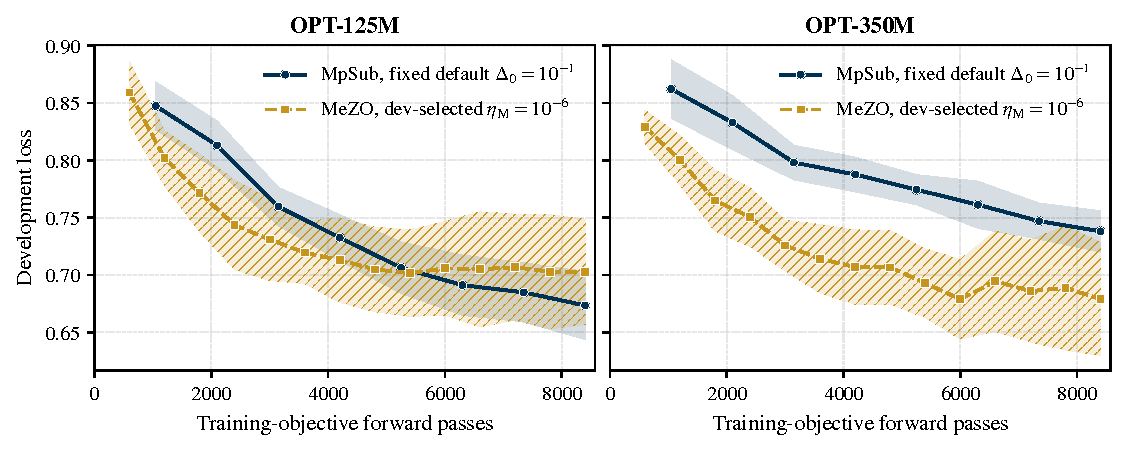
\includegraphics[width=0.90\textwidth]{fig_convergence_models.pdf}
\caption{Development loss versus training forward passes for OPT-125M (left) and OPT-350M (right), evaluated every 25 steps ($1{,}050$ forward passes) for \texttt{MpSub} and every 300 steps ($600$ forward passes) for MeZO. Curves show three-seed means; shaded bands indicate $\pm 1$ standard error of the mean.}
\label{fig:convergence}
\end{figure}

Figure~\ref{fig:sensitivity} compares the sensitivity of MeZO to its learning rate $\eta_{\mathrm{M}} \in [10^{-8}, 10^{-4}]$ with the sensitivity of \texttt{MpSub} to its initial radius $\Delta_0 \in \{10^{-3}, \allowbreak 10^{-2}, \allowbreak 3\times 10^{-2}, \allowbreak 10^{-1}, \allowbreak 3\times 10^{-1}\}$ on OPT-125M. Because MeZO holds $\eta_{\mathrm{M}}$ fixed throughout training, shifting $\eta_{\mathrm{M}}$ by one order of magnitude from $10^{-6}$ reduces mean test accuracy by $0.048$ at $10^{-7}$ and by $0.084$ at $10^{-5}$. In contrast, \texttt{MpSub} maintains a mean test accuracy between $0.655$ and $0.679$ across the $300$-fold range $\Delta_0 \in [10^{-3}, 3\times 10^{-1}]$. Because $\Delta_0$ serves only as the initial value for the geometric update \eqref{eq:radius_update_rule}, a small choice such as $\Delta_0 = 10^{-3}$ doubles on successful steps and reaches $\Delta_k \approx 10^{-1}$ within $\lceil \log_2(10^2) \rceil = 7$ iterations. Performance degrades only when $\Delta_0 \ge 1.0$ (mean test accuracies of $0.554$, $0.488$, and $0.464$ at $\Delta_0 \in \{1.0, 3.0, 10.0\}$), where the initial central-difference perturbations \eqref{eq:central_diff} incur large truncation error (Lemma~\ref{lem:fd_general}) and propose overly large initial steps.

\begin{figure}[htb]
\centering
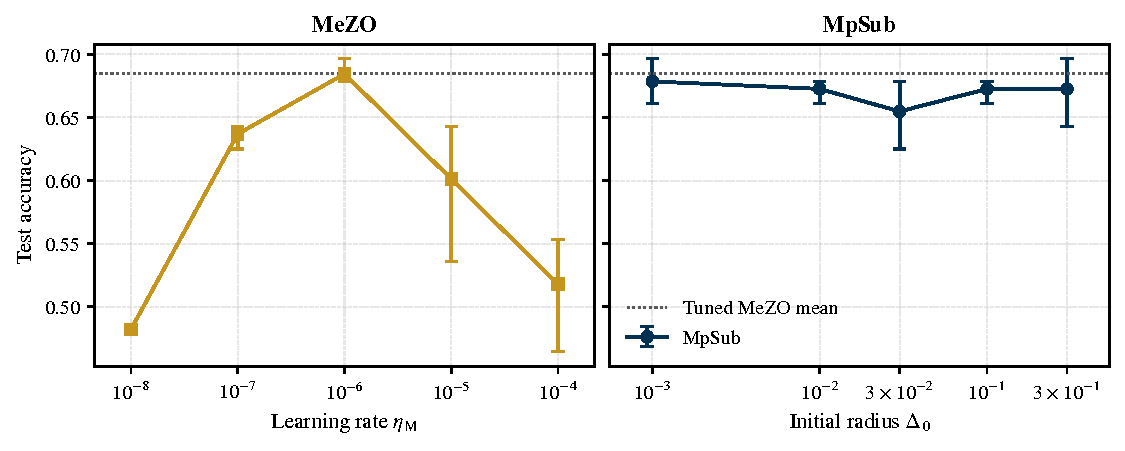
\includegraphics[width=0.90\textwidth]{fig_sensitivity.pdf}
\caption{Step-size sensitivity on OPT-125M under $8{,}400$ forward passes. Markers show three-seed mean test accuracy and vertical bars indicate min--max ranges. Left: MeZO across learning rates $\eta_{\mathrm{M}}$. Right: \texttt{MpSub} across initial radii $\Delta_0$; the horizontal dotted line marks the tuned MeZO mean ($0.685$).}
\label{fig:sensitivity}
\end{figure}

We next examine the effect of the subspace dimension $p \in \{5, 10, \allowbreak 15, \allowbreak 20, \allowbreak 25, \allowbreak 30\}$ on OPT-125M in Table~\ref{tab:p_ablation} under two protocols: (i) a fixed horizon of $100$ iterations (single seed) to measure per-iteration progress and wall-clock time, and (ii) a matched budget of at most $8{,}400$ forward passes across three seeds, under which \texttt{MpSub} executes $\lfloor 8{,}400/(2p+2)\rfloor$ iterations. At a fixed $100$-iteration horizon, increasing $p$ from $5$ to $20$ raises development accuracy from $0.700$ to $0.780$ and test accuracy from $0.643$ to $0.679$, consistent with the $(p-1)/n$ scaling in Lemma~\ref{lem:capture}, while per-step wall-clock time grows linearly with $2p+2$ from $3.0$\,s to $10.1$\,s. Under the fixed $8{,}400$-evaluation budget, smaller values of $p$ capture a smaller fraction of the gradient energy per iteration but execute more iterations ($700$ iterations at $p=5$ vs.\ $200$ at $p=20$); consequently, mean test accuracy remains within $0.667$--$0.685$ across all $p$, while $p \ge 20$ achieves higher mean development accuracy ($0.773$--$0.780$ vs.\ $0.740$--$0.760$ for $p \le 15$).

\begin{table}[htb]
\centering
\caption{Scaling with subspace dimension $p$ for OPT-125M on CommitmentBank ($\Delta_0 = 10^{-1}$). Left: fixed horizon of 100 steps (single seed, wall-clock time per step on an NVIDIA RTX 4060 Ti GPU). Right: matched budget of at most $8{,}400$ forward passes ($\lfloor 8{,}400/(2p+2)\rfloor$ steps; means and min--max ranges over three seeds).}
\label{tab:p_ablation}
\scriptsize
\begin{tabular}{@{}c@{\hspace{3.5pt}}c@{\hspace{3.5pt}}c@{\hspace{3.5pt}}c@{\hspace{3.5pt}}c@{\hspace{6pt}}c@{\hspace{3.5pt}}c@{\hspace{3.5pt}}c@{\hspace{3.5pt}}c@{}}
\toprule
& & \multicolumn{3}{c}{Fixed horizon (100 steps)} & \multicolumn{4}{c}{Matched budget ($\le 8{,}400$ passes, 3 seeds)} \\
\cmidrule(lr){3-5} \cmidrule(l){6-9}
$p$ & Fwd/step & Dev acc. & Test acc. & Time/step & Steps & Dev loss & Dev acc. & Test acc. \\
\midrule
5  & 12 & 0.700 & 0.643 & 3.0\,s & 700 & \begin{tabular}[c]{@{}c@{}}$0.670$ \\ ($0.592$--$0.743$)\end{tabular} & \begin{tabular}[c]{@{}c@{}}$0.760$ \\ ($0.720$--$0.820$)\end{tabular} & \begin{tabular}[c]{@{}c@{}}$0.685$ \\ ($0.679$--$0.696$)\end{tabular} \\ \addlinespace[3pt]
10 & 22 & 0.720 & 0.661 & 4.4\,s & 381 & \begin{tabular}[c]{@{}c@{}}$0.683$ \\ ($0.592$--$0.776$)\end{tabular} & \begin{tabular}[c]{@{}c@{}}$0.740$ \\ ($0.680$--$0.800$)\end{tabular} & \begin{tabular}[c]{@{}c@{}}$0.679$ \\ ($0.679$--$0.679$)\end{tabular} \\ \addlinespace[3pt]
15 & 32 & 0.740 & 0.661 & 6.0\,s & 262 & \begin{tabular}[c]{@{}c@{}}$0.673$ \\ ($0.607$--$0.751$)\end{tabular} & \begin{tabular}[c]{@{}c@{}}$0.747$ \\ ($0.720$--$0.780$)\end{tabular} & \begin{tabular}[c]{@{}c@{}}$0.667$ \\ ($0.661$--$0.679$)\end{tabular} \\ \addlinespace[3pt]
20 & 42 & 0.780 & 0.679 & 7.7\,s & 200 & \begin{tabular}[c]{@{}c@{}}$0.674$ \\ ($0.620$--$0.723$)\end{tabular} & \begin{tabular}[c]{@{}c@{}}$0.773$ \\ ($0.740$--$0.820$)\end{tabular} & \begin{tabular}[c]{@{}c@{}}$0.673$ \\ ($0.661$--$0.679$)\end{tabular} \\ \addlinespace[3pt]
25 & 52 & 0.780 & 0.679 & 8.7\,s & 161 & \begin{tabular}[c]{@{}c@{}}$0.676$ \\ ($0.610$--$0.738$)\end{tabular} & \begin{tabular}[c]{@{}c@{}}$0.773$ \\ ($0.740$--$0.820$)\end{tabular} & \begin{tabular}[c]{@{}c@{}}$0.673$ \\ ($0.661$--$0.679$)\end{tabular} \\ \addlinespace[3pt]
30 & 62 & 0.760 & 0.661 & 10.1\,s & 135 & \begin{tabular}[c]{@{}c@{}}$0.682$ \\ ($0.609$--$0.740$)\end{tabular} & \begin{tabular}[c]{@{}c@{}}$0.780$ \\ ($0.760$--$0.820$)\end{tabular} & \begin{tabular}[c]{@{}c@{}}$0.679$ \\ ($0.679$--$0.679$)\end{tabular} \\
\bottomrule
\end{tabular}
\end{table}

\subsection{Component ablation}
\label{subsec:component_ablation}

To evaluate \texttt{MpSub} in the smooth deterministic setting of Section~\ref{sec:analysis}, we minimize a $1{,}000$-dimensional nonquadratic function with rotated coordinates and power-law spectrum:
\begin{equation}
\label{eq:quartic_benchmark}
f(\bx) = \frac{1}{2}\sum_{j=1}^{n} \lambda_j z_j^2 + c_4 \sum_{j=1}^{n} \lambda_j^2 z_j^4,
\qquad \bz = (\bm I_n - 2\bm v\bm v^\top)(\bx - \bx_\star),
\end{equation}
where $n = 1{,}000$, $\lambda_j = 50 j^{-3/4}$ ($\lambda_1/\lambda_n \approx 280$), $c_4 = 0.05$, $\bm v \in \mathbb{R}^n$ is a fixed unit Householder vector, and $\bx_0 = \bm 0$. The optimizer accesses only function values $f(\bx)$, while exact gradients $\nabla f(\bx_k)$ are evaluated offline. Table~\ref{tab:component_ablation} reports the relative objective $f(\bx_K)/f(\bx_0)$, relative gradient norm $\|\nabla f(\bx_K)\|_2/\allowbreak\|\nabla f(\bx_0)\|_2$, and step acceptance rate after $8{,}400$ function evaluations across five random seeds.

\begin{table}[htb]
\centering
\caption{Component ablation on the smooth deterministic benchmark \eqref{eq:quartic_benchmark} ($n=1{,}000$, $8{,}400$ function evaluations; means and min--max ranges over five random seeds).}
\label{tab:component_ablation}
\footnotesize
\begin{tabular}{@{}l@{\hspace{3.5pt}}c@{\hspace{3.5pt}}c@{\hspace{3.5pt}}c@{\hspace{3.5pt}}c@{}}
\toprule
Variant & Steps & $f(\bx_K)/f(\bx_0)$ & $\|\nabla f(\bx_K)\|_2 / \|\nabla f(\bx_0)\|_2$ & Accept \\
\midrule
\texttt{MpSub} ($p=20, \Delta_0=10^{-1}$) & 200 & $0.158$ {\scriptsize($0.150$--$0.170$)} & $0.194$ {\scriptsize($0.184$--$0.219$)} & $0.58$ \\
\texttt{MpSub} + safeguard ($\kappa = 10^{-3}$) & 200 & $0.158$ {\scriptsize($0.150$--$0.170$)} & $0.194$ {\scriptsize($0.184$--$0.219$)} & $0.58$ \\
No momentum ($p=20$ random) & 200 & $0.186$ {\scriptsize($0.168$--$0.204$)} & $0.223$ {\scriptsize($0.211$--$0.231$)} & $0.58$ \\
Classical acceptance ($\rho_k \ge \eta$) & 200 & $0.188$ {\scriptsize($0.177$--$0.213$)} & $0.222$ {\scriptsize($0.209$--$0.267$)} & $0.50$ \\
\texttt{MpSub} ($p=2$ linear model) & 1,400 & $0.320$ {\scriptsize($0.296$--$0.330$)} & $0.288$ {\scriptsize($0.276$--$0.294$)} & $0.54$ \\
\midrule
\texttt{MpSub} from small $\Delta_0 = 10^{-3}$ & 200 & $0.174$ {\scriptsize($0.164$--$0.192$)} & $0.207$ {\scriptsize($0.194$--$0.223$)} & $0.58$ \\
\texttt{MpSub} from large $\Delta_0 = 1.0$ & 200 & $0.170$ {\scriptsize($0.158$--$0.180$)} & $0.205$ {\scriptsize($0.189$--$0.216$)} & $0.57$ \\
Fixed radius ($\Delta_k \equiv 10^{-3}$) & 200 & $0.667$ {\scriptsize($0.664$--$0.669$)} & $0.517$ {\scriptsize($0.511$--$0.520$)} & $1.00$ \\
Fixed radius ($\Delta_k \equiv 1.0$) & 200 & $1.000$ {\scriptsize($1.000$--$1.000$)} & $1.000$ {\scriptsize($1.000$--$1.000$)} & $0.00$ \\
\bottomrule
\end{tabular}
\end{table}

In the upper part of Table~\ref{tab:component_ablation}, we modify one component of \texttt{MpSub} at a time. Adding the expansion condition $\|\bg_k\|_2 \ge \kappa\Delta_k$ ($\kappa = 10^{-3}$) from \eqref{eq:safeguarded_radius} produces the exact same iterates as Algorithm~\ref{alg:mpsub} ($\kappa = 0$), because $\|\bg_k\|_2 \ge \kappa\Delta_k$ holds at every successful step during the $200$ iterations. Replacing the momentum direction $\bd_1^{(k)}$ with an independent Gaussian vector increases the final relative objective from $0.158$ to $0.186$ and the relative gradient norm from $0.194$ to $0.223$ with non-overlapping seed ranges ($0.150$--$0.170$ vs.\ $0.168$--$0.204$); as shown in \eqref{eq:expected_gaussian_capture}, retaining $\bd_1^{(k)}$ contributes the additional term $(\bm v_k^\top\bd_1^{(k)})^2$ to the expected squared norm of the projected gradient whenever the gradient correlates with the previous displacement. Reducing the subspace dimension from $p=20$ to $p=2$ ($1{,}400$ steps at $6$ evaluations per step) more than doubles the final relative objective ($0.320$ vs.\ $0.158$), while replacing the acceptance condition $\rho_k > 0$ in \eqref{eq:accept_rule} with the threshold $\rho_k \ge \eta$ discards descending trial steps with $0 < \rho_k < \eta$, reducing the acceptance rate from $0.58$ to $0.50$ and increasing the final relative objective to $0.188$.

In the lower part of Table~\ref{tab:component_ablation}, we compare the adaptive radius update \eqref{eq:radius_update_rule} with fixed trust-region radii. When $\Delta_k$ is held constant, $\Delta_k \equiv 10^{-3}$ accepts every step but makes slow progress ($f(\bx_K)/f(\bx_0) = 0.667$) because the step norm is restricted to $10^{-3}$, whereas $\Delta_k \equiv 1.0$ overshoots along the high-curvature directions of \eqref{eq:quartic_benchmark} and rejects every trial point ($1.000$). When $\Delta_k$ is updated via \eqref{eq:radius_update_rule}, \texttt{MpSub} initialized at either $\Delta_0 = 10^{-3}$ or $\Delta_0 = 1.0$ adjusts $\Delta_k$ within the first few iterations and reaches relative objectives of $0.174$ and $0.170$, close to the result obtained from $\Delta_0 = 10^{-1}$ ($0.158$).

\section{Conclusion}
\label{sec:conclusion}

We have presented \texttt{MpSub}, a momentum $p$-dimensional subspace trust-region method for high-dimensional derivative-free optimization and full-parameter language model fine-tuning. By combining the normalized displacement of the most recent accepted step with $p-1$ unorthogonalized Gaussian directions, \texttt{MpSub} relies on the near-orthonormality of high-dimensional Gaussian frames (Proposition~\ref{prop:gram_isometry}) to regenerate exploratory directions in place from scalar seeds, requiring only $\mathcal{O}(n)$ auxiliary memory and $2p+2$ function evaluations per iteration. For smooth deterministic objectives, we derived finite-difference error and single-step descent bounds for general non-orthogonal frames and proved unconditional almost-sure global convergence ($\lim_{k\to\infty} \|\nabla f(\bx_k)\|_2 = 0$) under a safeguarded radius update. Numerical experiments on a $1{,}000$-dimensional nonquadratic test problem and on SuperGLUE CommitmentBank fine-tuning of OPT-125M and OPT-350M demonstrated the practical contribution of each algorithmic component and showed that trust-region radius adaptation enables \texttt{MpSub} to match grid-searched MeZO using a single default configuration.

Several extensions merit further investigation. First, while our convergence analysis treats a deterministic objective $f$, language model fine-tuning evaluates a sampled minibatch objective $f_k$ at each iteration; extending the analysis of Section~\ref{sec:analysis} to stochastic minibatch evaluations under bounded variance is an important next step. Second, within each $p$-dimensional subspace $\mathcal S_k$, incorporating low-cost secant or diagonal curvature estimates---and parallelizing the $2p$ independent directional forward passes across devices---could further accelerate convergence while preserving the $\mathcal{O}(p)$ evaluation cost and $\mathcal{O}(n)$ memory footprint.

\begin{acknowledgements}
The authors thank the developers of the MeZO and LOZO codebases, on which the experimental infrastructure builds.
\end{acknowledgements}

\section*{Statements and Declarations}
The authors have no competing interests or funding to declare. The dataset analyzed during the current study is available in the SuperGLUE benchmark repository (\url{https://super.gluebenchmark.com}), and the source code for \texttt{MpSub} and the experiment scripts are available at \url{https://github.com/Julius-Valerius/MpSub}.

\bibliographystyle{spmpsci}
\bibliography{refs}

\end{document}
